\documentclass{article}
\usepackage{fullpage}
\usepackage{parskip}
\usepackage{standalone}
\usepackage{graphicx}
\usepackage{booktabs}
\usepackage{subcaption}
\usepackage{hyperref}
\usepackage{amsmath}
\usepackage{amsfonts}
\usepackage{amsthm}
\usepackage[table]{xcolor}
\usepackage{tikz}
\usetikzlibrary{arrows}
\usetikzlibrary{decorations.pathreplacing}
\usetikzlibrary{calc}
\usetikzlibrary{shapes.geometric}
\usetikzlibrary{decorations.markings}
\usetikzlibrary{shapes.geometric}
\usetikzlibrary{patterns,snakes}
\usetikzlibrary{decorations.text}
\usetikzlibrary{arrows.meta}

\usepackage{todonotes} %% for TODO notes


\newtheorem{theorem}{Theorem}


\title{Modelling Queues Where Customers Randomly Change Priority Classes While Waiting}
\author{Geraint I. Palmer, Michalis Panayidis \& Vincent Knight}
\date{}

\begin{document}
\maketitle

\section{Introduction}
There are a number of situations in which a customer's priority in a queue might
change during their time queueing, or equivalently where their priority depends
on the amount of time they have already spent in the queue.
Classic examples arise in healthcare systems, for example when a patient's
medical urgency might increase the longer they spend waiting due to health
degeneration. Another example would be a prioritisation scheme that attempts a
trade-off between medical need and waiting times.
These are both examples where a patient's priority has the chance to upgrade
over time while in the queue.
However there also might be situations in which a patient's priority can
downgrade over time: consider a medical intervention that can improve a
patient's outcome if caught early, if a patient has been waiting a long time
already then they might be passed over for a newly referred patient who will
gain more benefit from the intervention. In this case a patient's priority is
downgraded the longer they wait.

In this paper a single $M/M/c$ queue is modelled, with multiple classes of
customer of different priorities. While waiting in the queue customers change
their class to any other class at specific rates. Thus upgrades, downgrades, and
`skip-grades' (moving to a priority class not immediately above or below the
current class) are modelled.

This is first modelled using simulation, where we describe generalisable logic.
This is implemented in version v2.3.0 of the Ciw library in Python
\cite{palmer19}.
Then two Markov chain models are defined for the system, which are used to find
steady state distributions and expected sojourn times for each customer class.
These Markov chains give some insights into the behaviour of the systems under
different combinations of parameters; and numerical experiments give further
behaviours.

This paper is structured as follows:
Section~\ref{sec:system} defines the system under consideration in detail.
Section~\ref{sec:related} highlights some previous and related work.
Section~\ref{sec:simulation} discusses the contribution to the Ciw library and
the logic required to simulate this system.
Section~\ref{sec:makovchains} defines two Markov chain models of the system, one
useful for considering system-wide statistics such as state probabilities, and
one useful for considering customers' statistics such as average sojourn time.
Section~\ref{sec:bound} explores a bounded approximation for numerically
tractable analysis, and gives guidelines on choosing a large enough bound so as
to sufficiently approximate an unbounded system.
Section~\ref{sec:stationary} explores the parameter requirements for these
systems to have steady state distributions, and not grow infinitely.
Section~\ref{sec:behaviour} presents results from numerical experiments that
give insight into the behaviour of the system under various parameters.




\section{System Under Consideration}\label{sec:system}
Consider an $M/M/c$ queue with $K$ classes of customer labelled
$0, 1, 2, \dots, K-1$.
Let:

\begin{itemize}
  \item $\lambda_k$ be the arrival rate of customers of class $k$,
  \item $\mu_k$ be the service rate of customers of class $k$,
  \item $\theta_{i,j}$ be the rate at which customers of class $i$ change
  to customers of class $j$ while they are waiting in line.
\end{itemize}

Customers of class $i$ have priority over customers of class $j$ if $i < j$.
Customers of the same class are served in the order they arrived to that class.

Figure~\ref{fig:twoclass_example} shows an example with two classes of customer.

\begin{figure}
\begin{center}
\includestandalone[width=0.7\textwidth]{img/priority_queue}
\end{center}
\caption{An example of a two-class priority queue.}
\label{fig:twoclass_example}
\end{figure}

The key feature here is the $K \times K$ class change matrix
$\Theta = (\theta_{i,j})$. All elements $\theta_{i,j}$ where $i \neq j$ are
rates, and so are non-negative real numbers, if customers of class $i$ cannot
change to customers of class $j$ directly, then $\theta_{i,j} = 0$. The diagonal
values $\theta_{i,i}$ are unused as customers cannot change to their own class.
All elements $\theta_{i,i-1}$ represent the direct upgrade rates; all elements
$\theta_{i,i+1}$ represent the direct downgrade rates, while all other elements
can be thought of as `skip-grades`.
This is shown in Figure~\ref{fig:skipgrades}.

\begin{figure}
\begin{center}
\includestandalone[width=0.65\textwidth]{img/skipgrades}
\end{center}
\caption{Representations of parts of the matrix $\Theta$. Example when $K=5$.}
\label{fig:skipgrades}
\end{figure}




\section{Related Work}\label{sec:related}
Systems of this kind have been investigated previously:

\begin{itemize}
  \item \cite{jackson60} (1960): Non preemptive M/M/1 where customers
      are served in order of the difference between their waiting time
        and urgency number (that is priorities increasing linearly over
        time). Solved by considering event probabilities at clock ticks.
  \item \cite{holtzman71} (1971): Similar to the above, but treat each
      urgency number as a separate customer class, and not considering
        clock ticks. Upper and lower bounds on the waiting times, based
        on FIFO and static priorities.
  \item \cite{netterman79} (1979): Now considers the case where
      priorities increase non-linearly but concavely over time.
  \item \cite{fratini90} (1990): Non preemptive M/G/1 queue with two
      classes of customers, where priorities switch if the number from
        one class exceeds a given threshold. Lower priority customers
        have a finite waiting capacity, higher have infinite capacity.
  \item \cite{knessl03} (2003): Similar to the above but with Markovian
      services and infinite waiting capacities for both customers.
  \item \cite{xie08} (2008): Preemptive n-priority-classes M/M/c with
      exponential upgrades. Customers only upgrade to the priority
        immediately higher than themselves. Stability considered.
  \item \cite{down10} (2010): Preemptive two-priority-classes M/M/c with
      exponential upgrades. Customers cannot upgrade if the number of
        lower priority customers is below a given threshold. Holding
        costs considered.
  \item \cite{he12} (2012): Extension of the above, allows batch
      arrivals, multiple classes, phase-type upgrades and services.
        Customers only upgrade to the priority immediately higher than
        themselves.
  \item \cite{bilodeau22} (2022): Analytical (truncated) expressions for
      a two class delayed accumulating priority M/G/1 queue. Customer
        priorities increase linearly over time, at different rates
        according to class, after an initial fixed delay.
\end{itemize}

\todo[inline]{Add more literature, flesh out as paragraphs.}



\section{Simulation Model Logic}\label{sec:simulation}
The Ciw library \cite{palmer19} is an open-source Python library for
discrete-event simulation of open queueing networks. A key contribution of this
work is the adaptation of the library's logic to facilitate the type of
dynamically changing priority classes described in Section~\ref{sec:system}.
This adaptation is released in version Ciw v2.3.0, with usage documentation at
\url{https://ciw.readthedocs.io/en/latest/Guides/change-class-while-queueing.html}.

The core of Ciw's logic is the event scheduling approach, described in
\cite{robinson14}. This is a variant of the three-phase approach, with an
\textbf{A}-phase which advances the clock to the next scheduled event, a
\textbf{B}-phase where scheduled events are carried out, and a \textbf{C}-phase
where conditional events are carried out. Figure~\ref{fig:eventscheduling} shows
a flow diagram of the logic of the event scheduling approach.

\begin{figure}
    \centering
    \includestandalone[width=0.25\textwidth]{img/eventschedulingapproach}
    \caption{Flow diagram of the event scheduling approach used by Ciw, taken from \cite{palmer18}.}
    \label{fig:eventscheduling}
\end{figure}

The primary scheduled, or \textbf{B}-events are customers arriving to a queue,
and customers finishing service. The conditional, or \textbf{C}-events are those
that happen immediately after, and because of, these \textbf{B}-events. The
primary ones are customers beginning service, and customers leaving the queue.

All other features of queueing systems that can be simulated with the Ciw
library involve increasing the range of \textbf{B}- and \textbf{C}-events that
can happen during the simulation run.
In the case of customers randomly changing priority classes while waiting, one
additional \textbf{B}-event and one additional \textbf{C}-event are included:

\begin{itemize}
  \item Upon arrival to the queue customers are assigned a date in which they
  will change customer class, determined by randomly sampling from a
  distribution. Therefore each customer's event of changing customer class is
  scheduled for the future, and are therefore \textbf{B}-events. If those
  customers begin service (which might not be scheduled yet) before that event
  has occurred, then their changing customer class event is cancelled.
  \item Upon changing class, they immediately schedule another changing class
  event for the future, again sampling a date from a given distribution. This
  happens immediately after the above, and so is a \textbf{C}-event.
\end{itemize}

Note that the particular distributions used to sample class change dates in
these cases are generic, and any of Ciw's currently pre-programmed distributions
can be chosen, or custom distributions can also be input. For the systems
described in this paper, we choose Exponential distributions with rates
determined by the class change matrix $\Theta$.




\section{Markov Chain Models}\label{sec:makovchains}
The situation described in words in Section~\ref{sec:system} can be described
precisely as two different Markov chains.
The first, described in Section~\ref{sec:state_formulation}, describes the
overall changes in state, where a state records the number of customers of each
class at the node. This is useful for analysing system-wide statistics such as
average queue size.
The second, described in Section~\ref{sec:sojourn_formulation}, describes how an
individual arriving customer experiences the system until their exit. This is
useful for analysing individual customers' statistics such as average sojourn
time.


\subsection{Discrete State Markov Chain Formulation}\label{sec:state_formulation}
Let
$\underline{\mathbf{s}}_t = (s_{0,t}, s_{1,t}, \dots, s_{K-1,t}) \in \mathbb{N}^K$
represent the state of the system at time step $t$, where $s_{k,t}$ represents
the number of customers of class $k$ present at time step $t$.

Then the rates of change between $\underline{\mathbf{s}}_t$ and
$\underline{\mathbf{s}}_{t+1}$ are given by Equation~\ref{eqn:transitions},
where $\underline{\mathbf{\delta}} = \underline{\mathbf{s}}_{t+1} - \underline{\mathbf{s}}_t$,

\begin{equation}\label{eqn:transitions}
q_{\underline{\mathbf{s}}_t, \underline{\mathbf{s}}_{t+1}} = 
\begin{cases}
\lambda_k & \text{if } \delta_k = 1 \text{ and } \delta_i = 0 \; \forall \; i \neq k \\
B_{k,t} \mu_k & \text{if } \delta_k = 1 \text{ and } \delta_i = 0 \; \forall \; i \neq k \text{ and } \sum_{i < k} s_{i,t} < c \\
(s_{k,t} - B_{k,t}) \theta_{k_0,k_1} & \text{if } \delta_{k_0} = -1 \text{ and } \delta_{k_1} = 1 \text{ and } \delta_i = 0 \; \forall \; i \neq k_0, k_1 \\
0 & \text{otherwise.}
\end{cases}
\end{equation}

and $B_{k,t}$, representing the number of customers of class $k$ currently in
service at time step $t$, is given by Equation~\ref{eqn:inservice}, where $c$
is the number of servers.

\begin{equation}\label{eqn:inservice}
B_{k,t} =\min\left(c - \min\left(\sum_{i < k} s_{i,t}, c\right), s_{k,t}\right)
\end{equation}




\subsection{Sojourn Time Markov Chain Formulation}\label{sec:sojourn_formulation}
Let $\underline{\mathbf{z}}_t = (z_{0,t}, z_{1,t}, \dots, z_{n,t} \dots, z_{K-1,t}, m_t, n_t) \in \mathbb{N}^{K+2}$
represent the state of a particular customer at time step $t$, where $n_t$
represents that customer's class at time $t$; $z_{k,t} \; \forall \; k < n$
represents the number of customers of class $k$ in front of the customer in the
queue at time $t$; $z_{k,t} \; \forall \; n < k < K$ represents the number of
customers of class $k$ behind the customer in the queue at time $t$; and $m_t$
represent the number of customers of class $n_t$ behind the customer in the
queue at time $t$.
Also let $\star$ represent an absorbing state, representing the state where that
customer has finished service and left the system.

Then the rates of change between $\underline{\mathbf{z}}_t$ and
$\underline{\mathbf{z}}_{t+1}$ are given by Equation~\ref{eqn:transitions_sojourn},
where $\underline{\mathbf{\delta}} = \underline{\mathbf{z}}_{t+1} - \underline{\mathbf{z}}_t$,

\begin{equation}\label{eqn:transitions_sojourn}
\resizebox{\textwidth}{!}{%
$q_{\underline{\mathbf{z}}_t, \underline{\mathbf{z}}_{t+1}} = 
\begin{cases}
\mu_n & \text{if } z_{t+1} = \star \text{ and } \sum_{k \leq n} z_{k, t} < c \\
\lambda_n & \text{if } \delta_K = 1 \text{ and } \delta_i = 0 \; \forall \; i \neq K \\
\lambda_k & \text{if } \delta_k = 1 \text{ and } \delta_i = 0 \; \forall \; i \neq k \text{ and } k \neq n\\
A_{k,n,t} \mu_k & \text{if } \delta_k = -1 \text{ and } \delta_i = 0 \; \forall \; i \neq k \text{ and } k < K\\
\tilde{A}_{n,t} \mu_n & \text{if } \delta_K = -1 \text{ and } \delta_i = 0 \; \forall \; i \neq K\\
(z_{k_0,t} - A_{k_0,n,t}) \theta_{k_0,k_1} & \text{if } \delta_{k_0} = -1 \text{ and } \delta_{k_1} = 1 \text{ and } \delta_i = 0 \; \forall \; i \neq k_0, k_1 \text{ and } k_0 < K \text{ and } k_1 \neq n, K, K+1 \\
(z_{K,t} - \tilde{A}_{n,t}) \theta_{n,k} & \text{if } \delta_K = -1 \text{ and } \delta_{k} = 1 \text{ and } \delta_i = 0 \; \forall \; i \neq k, n \text{ and } k < K \\
(z_{k,t} - A_{k,n,t}) \theta_{k,n} & \text{if } \delta_k = -1 \text{ and } \delta_K = 1 \text{ and } \delta_i = 0 \; \forall \; i \neq k, K \\
\theta_{n, k} & \text{if } \delta_n = z_{K,t} \text{ and } \delta_K = -z_{K,t} \text{ and } \delta_{K+1} = n - k \text{ and } \delta_i = 0 \text{ otherwise, and } \sum_{k \leq n} z_{k, t} < c \\
0 & \text{otherwise.}
\end{cases}$%
}
\end{equation}

and $A_{k,n,t}$ and $\tilde{A}_{n, t}$, representing the number of customers of
class $k$ currently in service, are given by Equations~\ref{eqn:inservice_adapt}
and~\ref{eqn:inservice_adapt_tilde}.

\begin{equation}\label{eqn:inservice_adapt}
A_{k,n,t} =
\begin{cases}
\min\left(c, \sum_{i \leq k} z_{i,t}\right) - \min\left(c \sum_{i < k} z_{i,t}\right) & \text{if } k \leq n \\
\min\left(c, \sum_{i \leq k} z_{i,t} + 1 + z_{K,t}\right) - \min\left(c \sum_{i < k} z_{i,t} + 1 + z_{K,t}\right) & \text{if } n < k < K
\end{cases}
\end{equation}

\begin{equation}\label{eqn:inservice_adapt_tilde}
\tilde{A}_{n,t} =
\min\left(c, \sum_{i \leq n} z_{i,t} + 1 + z_{K,t}\right) - \min\left(c, \sum_{i \leq n} z_{i,t} + 1\right) \\
\end{equation}


The expected time to absorption can be calculated from each state.
Customers arrive in all states where $z_{K,t} = 0$, and their class can be
determined by $n$. Combining these times to absorption with the state
probabilities found in the previous section, the sojourn times for each customer
class can be found.




\section{Bounded Approximation}\label{sec:bound}
In order to analyse the above Markov chain models numerically, finite
approximations can be made. Define $b$ as a bound, such that the maximum allowed
number of customers of each priority class is $b$, with transitions to any
states greater than this disallowed.
Assuming the infinite system reaches a stationary distribution, then the
probability of the number of customers of a particular customer class exceeding
$b$ approaches zero as $b$ increases. Thus the finite approximations approaches
a good approximation as $b$ increases, and any statistics found using a bounded
approximation will approach their corresponding values of the infinite models as
$b$ increases.

\todo[inline]{Reword this and justify better.}

Choosing an appropriate value for $b$ is a trade off between accuracy and model
size, and so computational time. An inefficient way to choose $b$ would be to
sequentially build bounded models, increasing $b$ each time, calculating the
statistics of interest, and observing when the relationship between $b$ and that
statistic levels off.
It would be more efficient to choose a $b$ and be able to immediately check if
the accuracy is sufficient. We propose two checks, one for ergodic Markov
chains (the model in Section~\ref{sec:state_formulation}), and one for absorbing
Markov chains (the model in Section~\ref{sec:sojourn_formulation}).




\subsection{Bound check for ergodic Markov chains}\label{sec:ergodic_check}
Let $S_b = \{\underline{\mathbf{s}} \in S \;|\; b \in \underline{\mathbf{s}}\}$, the
set of states that lie on the Markov chain boundary. We wish to choose $b$ large
enough that the boundary is irrelevant, that is that the Markov chain hardly
ever reaches the boundary. Consider
$\max_{\underline{\mathbf{s}} \in S_b} \pi_{\underline{\mathbf{s}}}$, the
largest of the steady-state probabilities of being at a state on the boundary.
Choose a tolerance level $\epsilon > 0$. Now consider $b$ large enough if

\begin{equation}
\max_{\underline{\mathbf{s}} \in S_b} \pi_{\underline{\mathbf{s}}} < \epsilon.
\end{equation}

As an example, consider a standard M/M/1 queue with arrival rate $\lambda = 4$
and service rate $\mu = 5$.
Here the set $S_b$ contains just one state, the state $b$.
Figure~\ref{fig:ergodic_b7} shows the steady state probabilities obtained when
$b=7$, while Figure~\ref{fig:ergodic_b39} shows the steady state probabilities
obtained when $b=39$; both choosing $\epsilon=0.02$.
Under the proposed check it can be seen that $b=7$ is not sufficient to
approximate an infinite system as $\pi_7 > \epsilon$, while $b=39$ is sufficient
as $\pi_{39} < \epsilon$.

\begin{figure}[!htbp]
  \begin{center}
  \begin{subfigure}[b]{0.65\textwidth}
    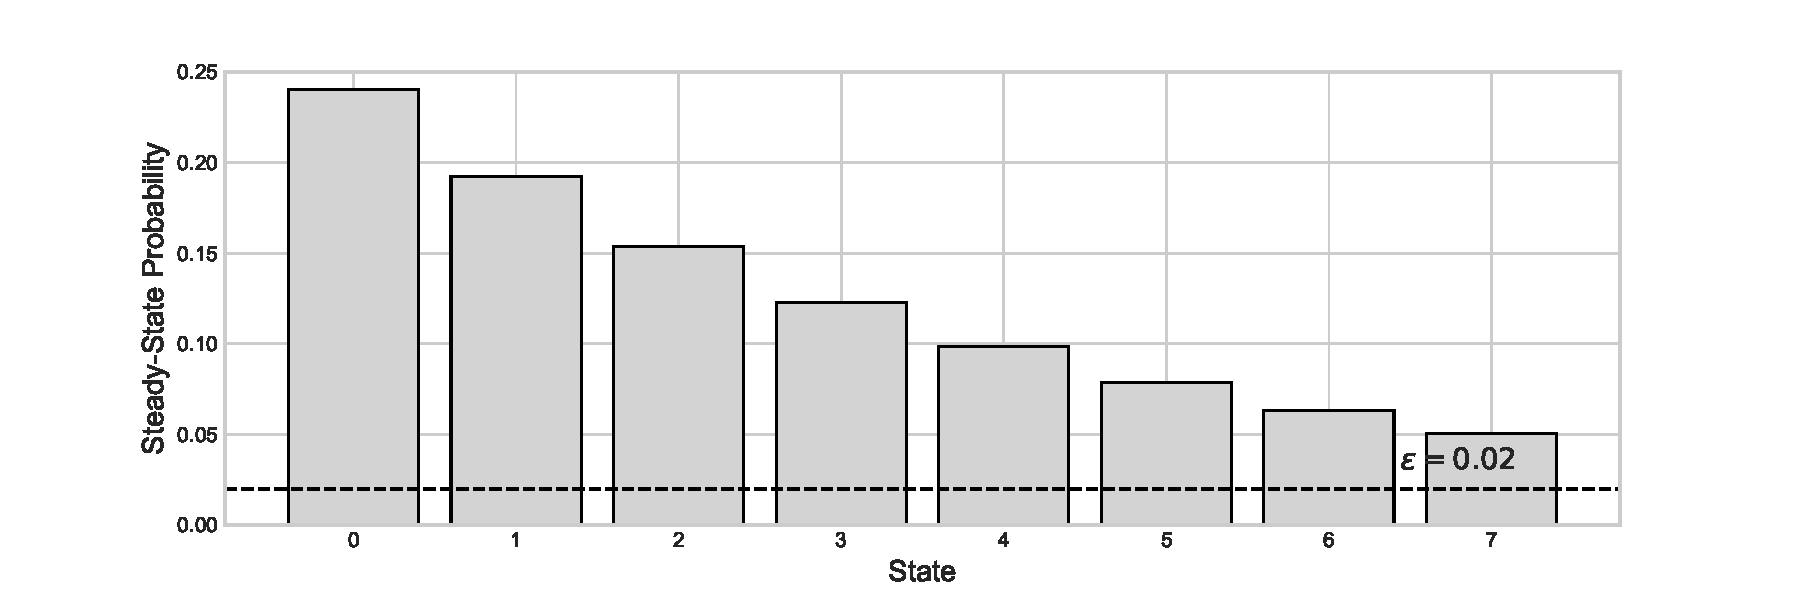
\includegraphics[width=\textwidth]{img/example_mc_8states.pdf}
    \caption{$b=7$}
    \label{fig:ergodic_b7}
  \end{subfigure}
  \begin{subfigure}[b]{0.65\textwidth}
    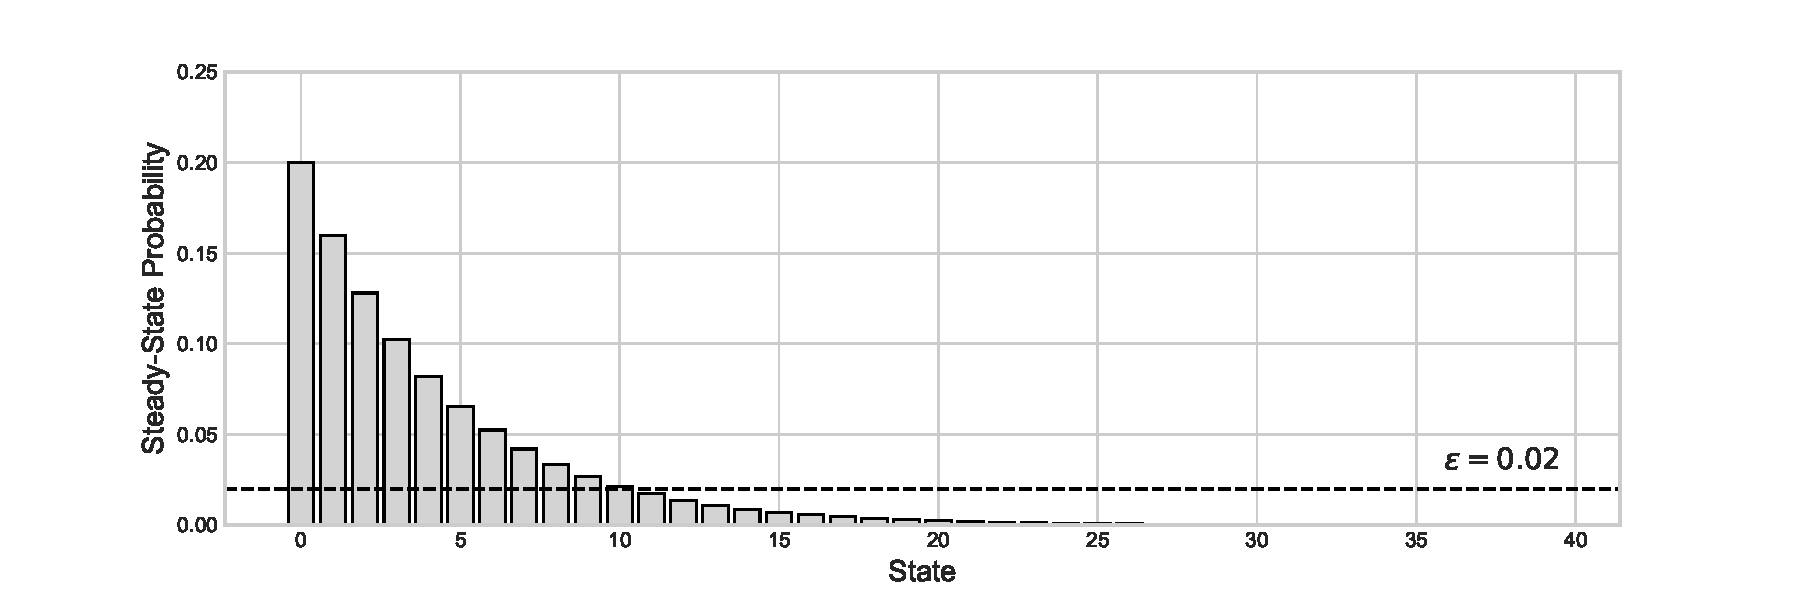
\includegraphics[width=\textwidth]{img/example_mc_40states.pdf}
    \caption{$b=39$}
    \label{fig:ergodic_b39}
  \end{subfigure}
  \end{center}
  \caption{Steady-state probabilities of bounded approximations of an M/M/1
  queue.}
  \label{fig:ergodic_check}
\end{figure}

\todo[inline]{Add a plot of max $\max \pi_s - \epsilon$ as a function of $b$.}



\subsection{Bound check for absorbing Markov chains}\label{sec:absorbing_check}
The above check isn't possible for absorbing Markov chains as they will not
reach steady state, so another check is required. This method assumed the
absorbing Markov chain takes the same shape as defined in
Section~\ref{sec:sojourn_formulation}, where states move further away from the
absorbing state as their labels increase.

Again let $S_b = \{\underline{\mathbf{s}} \;|\; b \in \underline{\mathbf{s}}\}$,
the set of states that lie on the Markov chain boundary. Now define $h_{i,J}$ as
the hitting probabilities of a set of states $J$ from state $i$, that is, what
is the probability of ever reaching any state in $J$ when starting from state
$i$. These are defined recursively as:

\begin{equation}
h_{iJ} = \begin{cases}
\sum_k p_{ik} h_{kJ} & \text{if } i \notin J \\
1 & \text{if } i \in J
\end{cases}
\end{equation}

Now for the bounded approximation define a \textit{reasonable region}, $R$, of
the state space, a region of states which we reasonable expect the infinite
Markov chain to visit. Let it's complement be known as the \textit{unreasonable
region}.
Let us define $R$ by the percentage $r$ of the distance between the absorbing
state and a boundary state, that is
$R = \{\underline{\mathbf{s}} \;|\; \lVert \mathbf{s} \rVert < rb \text{ for all } s \in \underline{\mathbf{s}}\}$,
where $\lVert \mathbf{x} \rVert = \sum_i x_i$.

Now as above, choose a tolerance level $\epsilon > 0$. Now consider $b$ large
enough if

\begin{equation}
\max_{\underline{\mathbf{s}} \in R} h_{\underline{\mathbf{s}} S_b} < \epsilon.
\end{equation}

As an example, consider a standard M/M/1 queue, with arrival rate $\lambda = 4$
and service rate $\mu = 5$, but with arrivals rejected if the queue is empty.
That is the state $0$ is an absorbing state, see Figure~\ref{fig:mm1_absorbing}.
Here the set $S_b$ contains just one state, the state $b$.
Figure~\ref{fig:absorbing_b7} shows the hitting probabilities from each state to
$b$ obtained when $b=7$, while Figure~\ref{fig:absorbing_b39} shows the hitting
probabilities obtained when $b=39$; both choosing $\epsilon=0.05$ and $r=0.75$.
Under the proposed check it can be seen that $b=7$ is not sufficient to
approximate an infinite system as $h_{5,7} > \epsilon$, while $b=39$ is
sufficient as $h_{29, 39} < \epsilon$.

\begin{figure}
\includestandalone[width=\textwidth]{img/absorbing_mm1}
\caption{An M/M/1 queue with absorbing state.}
\label{fig:mm1_absorbing}
\end{figure}

\begin{figure}[!htbp]
  \begin{center}
  \begin{subfigure}[b]{0.65\textwidth}
    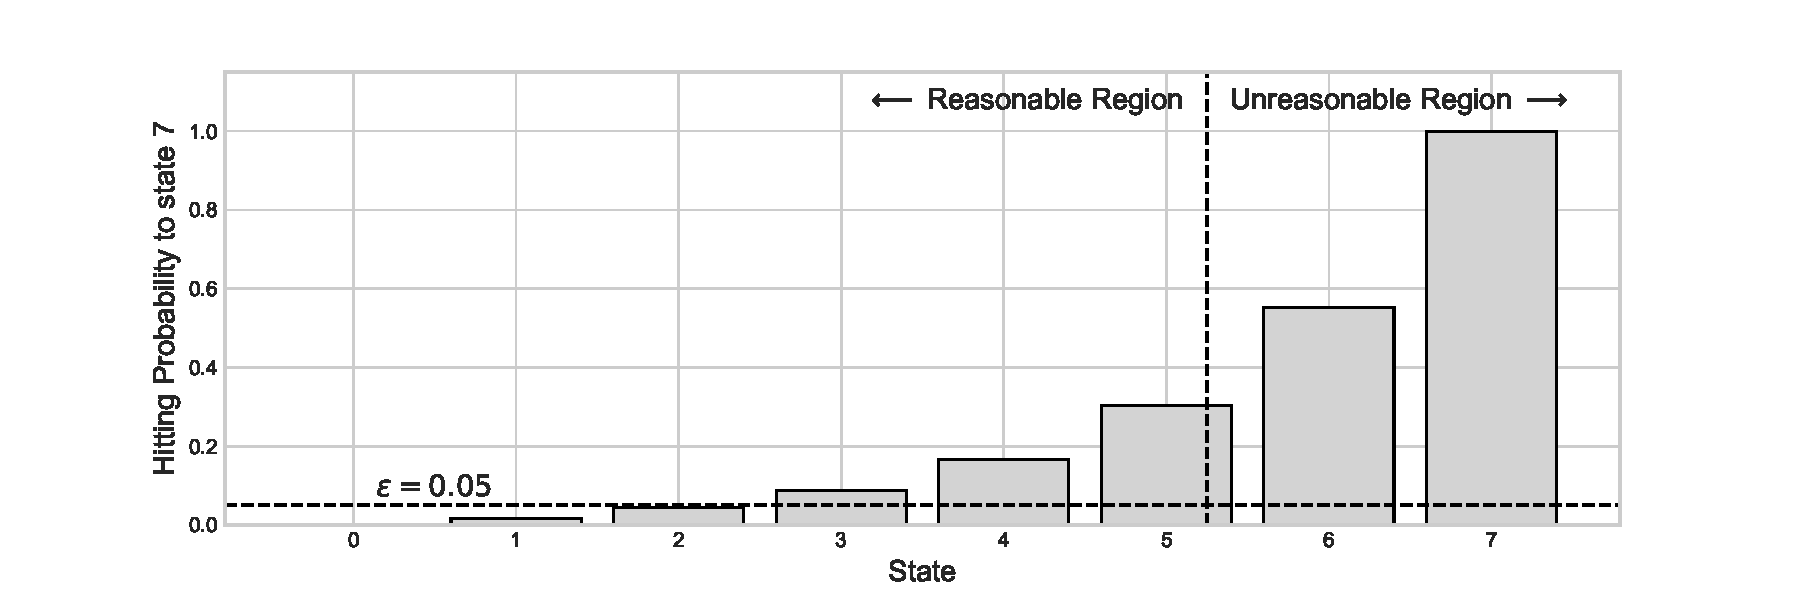
\includegraphics[width=\textwidth]{img/example_absorbingmc_8states.pdf}
    \caption{$b=7$}
    \label{fig:absorbing_b7}
  \end{subfigure}
  \begin{subfigure}[b]{0.65\textwidth}
    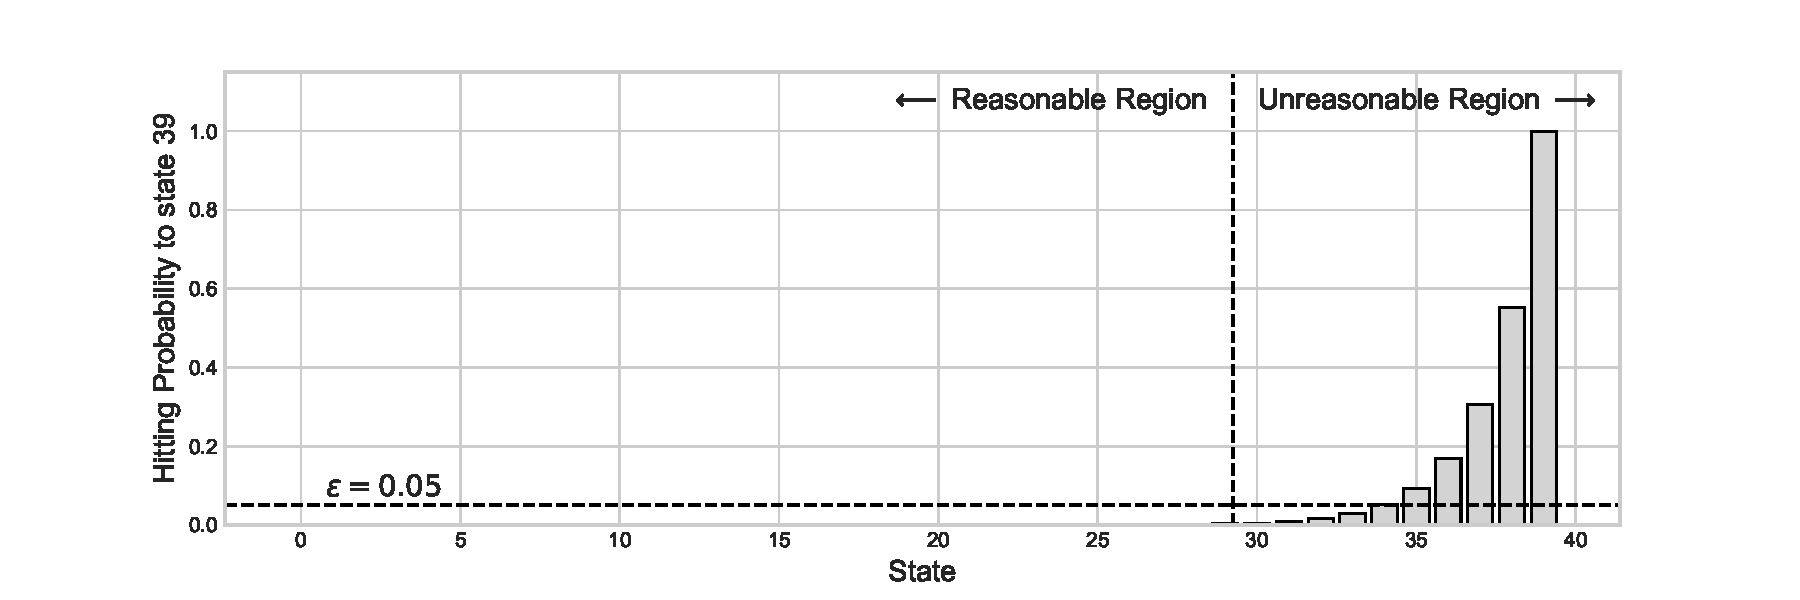
\includegraphics[width=\textwidth]{img/example_absorbingmc_40states.pdf}
    \caption{$b=39$}
    \label{fig:absorbing_b39}
  \end{subfigure}
  \end{center}
  \caption{Hitting probabilities of bounded approximations of an absorbing
  M/M/1 queue.}
  \label{fig:absorbing_check}
\end{figure}

\todo[inline]{Add a plot of max $\max h - \epsilon$ as a function of $b$.}


The hyperparameters choices of $\epsilon$ and $r$ can greatly effect the
effectiveness of this check, and aren't as intuitive as the boundary hitting
tolerance hyperparameter of Section~\ref{sec:ergodic_check}. In general,
increasing $r$ increases the relative size of the reasonable region, and so a
larger bound would be needed to ensure a low hitting probability from this
region to the boundary. Decreasing $\epsilon$ forces the probability of hitting
the boundary from the reasonable region to be smaller, and so a larger boundary
would be needed.

To investigate, consider an arbitrarily chosen statistic for the example system
described above, the mean time to absorption from state 6.
Figure~\ref{fig:investigate_hyperparameters} shows this calculated value using
different values of the boundaries $b$, and highlights the boundaries that were
accepted or rejected by this check for combinations of $\epsilon = 0.01, 0.02$
and $0.05$, and $r = 0.6, 0.7, 0.8$ and $0.9$.
As the mean time to absorption levels off we can be confident that the bound is
large enough to approximate the infinite system; and as both $r$ and $\epsilon$
increase the check will only accept bounds that are large enough.

\begin{figure}
  \begin{center}
    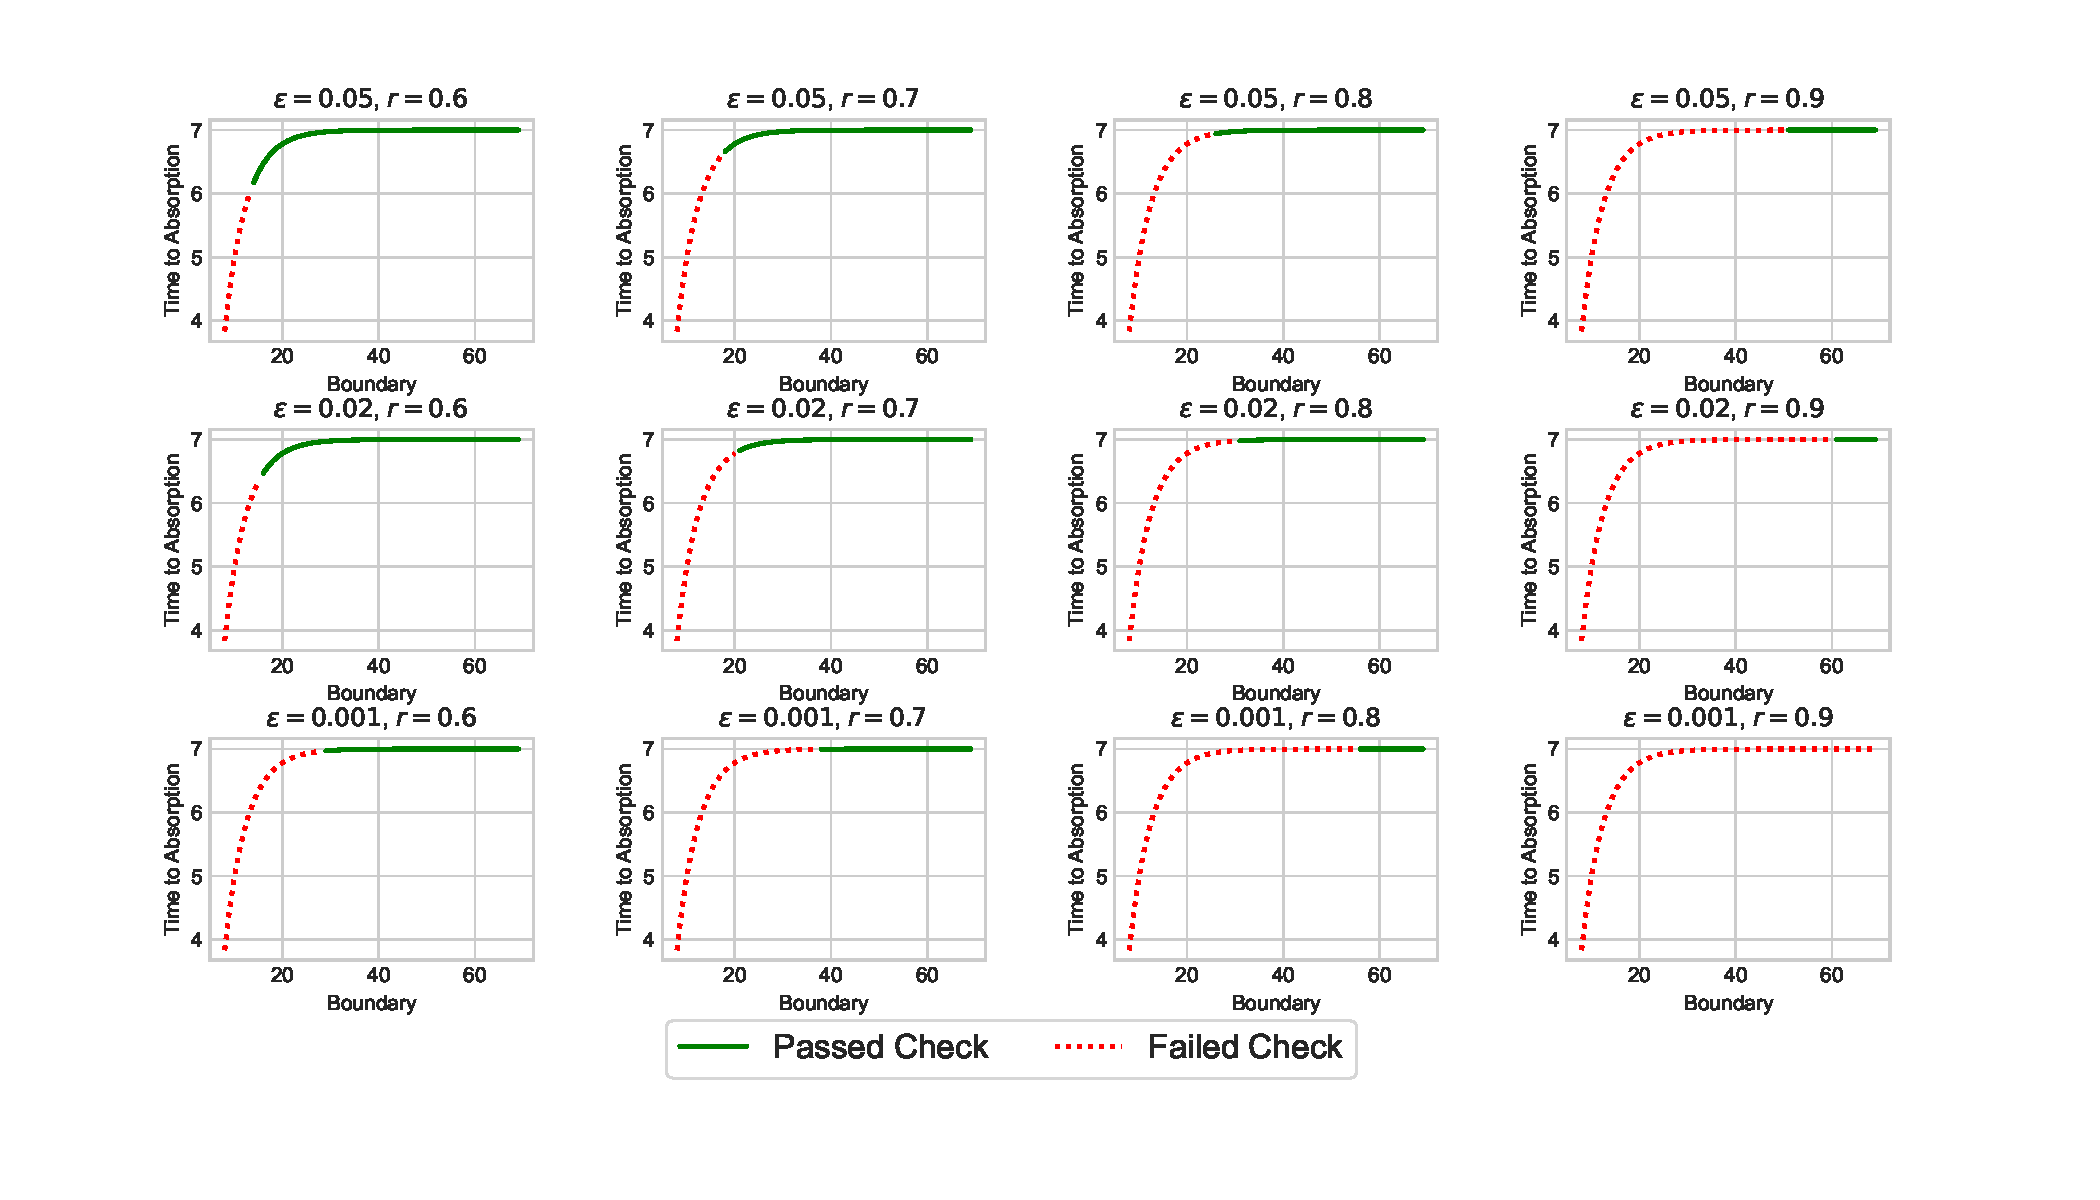
\includegraphics[width=0.8\textwidth]{img/check_hyperparameters_effect.pdf}
  \end{center}
  \caption{Investigating the effect of the hyperparameters $\epsilon$ and $r$.}
  \label{fig:investigate_hyperparameters}
\end{figure}

However this is a trade-off between accuracy and model size.
This is highlighted further in Figure~\ref{fig:summary_hyperparameters}.
This plot on the left shows the minimum $b$ required to pass the check with the
given hyperparameters $\epsilon$ and $r$; and the plot on the right shows the
absolute error between the result obtained from using that minimum bound and the
infinite system (the infinite system here is modelled as a bounded system with a
very large bound of $b = 200$).

\begin{figure}
  \begin{center}
    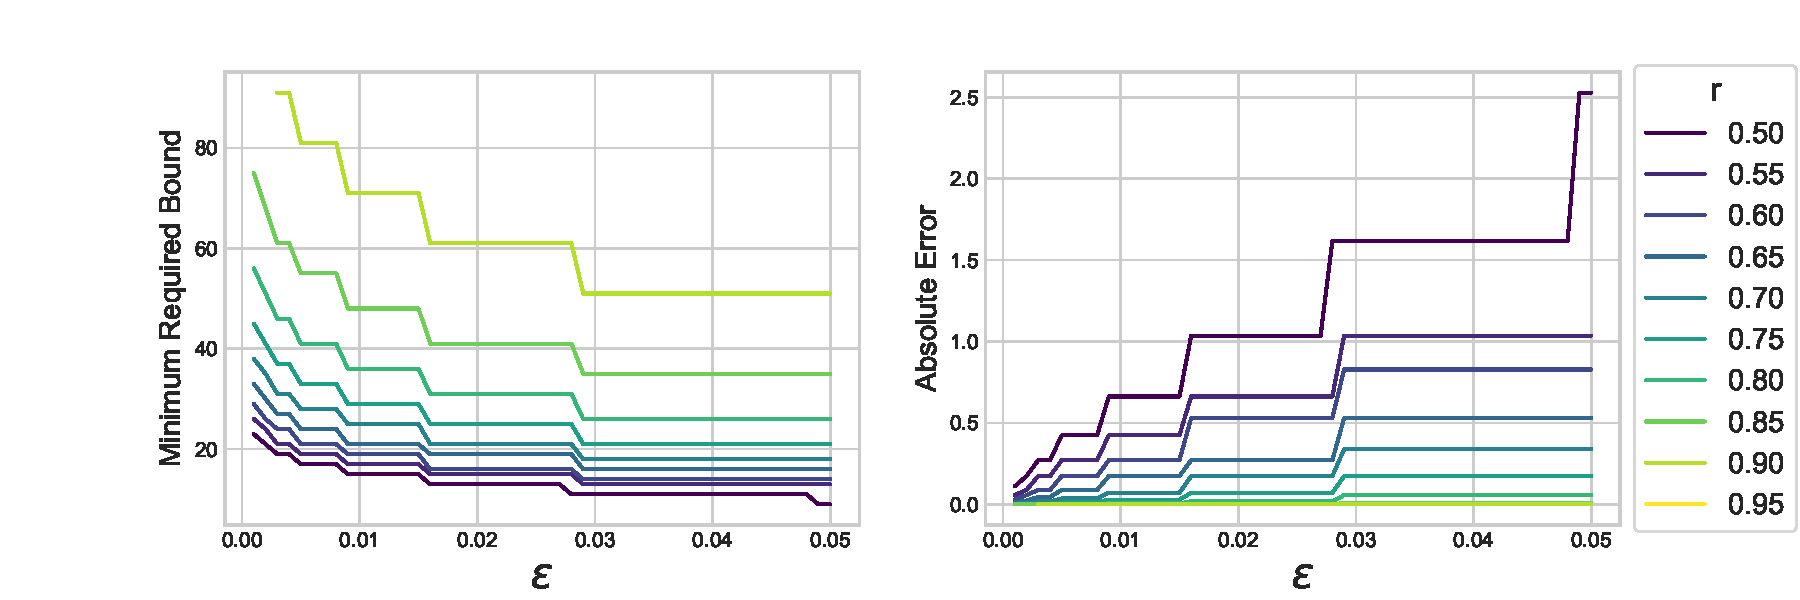
\includegraphics[width=0.9\textwidth]{img/check_hyperparameters_effect_summary.pdf}
  \end{center}
  \caption{Investigating the effect of the hyperparameters $\epsilon$ and $r$ on
  accuracy and model size.}
  \label{fig:summary_hyperparameters}
\end{figure}




\section{Existence of Stationary Distributions}\label{sec:stationary}
A key difference between using a bounded approximation to analysing infinite
Markov chains is the existence of stationary distributions. All bounded
approximations have steady state distributions, even if the corresponding
infinite Markov chain does not, leading to spurious results in these cases.
Theorem~\ref{thrm:steadystate} gives a naive check for the existence or
non-existence of steady states, but does not cover all possibilities.

\begin{theorem}\label{thrm:steadystate}
For an $M/M/c$ work conserving queue with $K$ classes of customer, with arrival
rate and service rate $\lambda_k$ and  $\mu_k$ for customers of class $k$,
respectively; then
\begin{enumerate}
  \item it will reach steady state if $\sum_i \lambda_i < c \min_i \mu_i$ ,
  \item it will never reach steady state if $\sum_i \lambda_i > c \max_i \mu_i$.
\end{enumerate}
\end{theorem}

Note that this result does not assume any particular service discipline such as
first-in-first-out or prioritised classes, but holds for any work conserving
discipline.

\begin{proof}
The queue will reach steady state if the rate at which customers are added to
the queue is less than the rate at which customers leave the queue.
As arrivals are not state dependent, customers are added to the queue at a rate
$\sum_i \lambda_i$ when in any state.
The rate at which customers leave the queue is state dependent, depending on the
service discipline.

We do not need to consider cases when there are less than $c$ customers present,
as here any new arrival will increase the rate at which customers leave the
queue, as that arrival would enter service immediately.
Considering the cases where there are $c$ or more customers in the queue, there
are two extreme cases, either:

\begin{enumerate}
  \item all customers in service are of the class with the slowest service rate.
  In this case the rate at which customers leave the queue is $c \min_i \mu_i$,
  which is the slowest possible rate at which customers can leave the queue.
  If $\sum_i \lambda_i < c \min_i \mu_i$ then the rate at which customers enter
  the queue is smaller than the smallest possible rate at which customers leave
  the queue, and so will always be smaller than the rate at which customers
  leave the queue in all states. Therefore the system will reach steady state.
  Or:
  \item all customers in service are of the class with the fastest service rate.
  In this case the rate at which customers leave the queue is $c \max_i \mu_i$,
  which is the fastest possible rate at which customers can leave the queue.
  If $\sum_i \lambda_i > c \max_i \mu_i$ then the rate at which customers enter
  the queue is greater than the largest possible rate at which customers leave
  the queue, and so will always be greater than the rate at which customers
  leave the queue in all states. Therefore the system cannot reach steady state.
\end{enumerate}
\end{proof}

If $c \min_i \mu_i < \sum_i \lambda_i < c \max_i \mu_i$ then more investigation
is needed. In the case of dynamic priority classes the class change matrix
$\Theta$ may be significant. For example the service rate of customers of one
class may be very slow, however if the rate at which customers leave that class
is sufficiently large then that service rate may not have an effect.
Alternatively if the rate at which customers of the other classes change to that
class is large, then that slow service rate could be a bottleneck for the
system.

\todo[inline]{Add the above as numerical examples with plots?}

\todo[inline]{Can we think of any way of investigating this?}




\section{Effect of $\Theta$ on System Behaviour}\label{sec:behaviour}

\todo[inline]{Design and run numerical experiments using checks above to keep
the Markov chains accurate but of reasonable size.}


\bibliographystyle{plain}
\bibliography{refs}

\end{document}
